In order to understand the requirement of testing within DataOps, it is important to understand the principles and processes of DataOps itself. In general, DataOps is an approach within building and conducting data analytics which combines established methodologies originating from DevOps, \ac{spc} as well as \textit{agile} software development \cite[24]{Bergh2019}. Several components from each of these methodologies are taken and applied to building and conducting data analytics. These processes aim to eliminate analytics issues found in the traditional development process of such solutions. These issues include but are not limited to slow development and adaptation of analytics solutions \cite{Lockner2019}, error-prone analytics results, repetitive manual processes \cite[11\psqq]{Bergh2019}, etc. Testing is a common component that supports these DataOps processes.

During the rise of DataOps, other terms, including \textit{\acs{ml}Ops}, \textit{\acs{ai}Ops}, etc., emerged. It is to mention that all data-related \textit{Ops} underlie the general DataOps methodology and focus on specific subsets of data analytics applications \cite{Aslett2018}.

\subsection{\acs{spc} Heritage: Data Analytics Pipeline}
Common data analytics solutions work by means of a pipeline: Data is acquired from various sources and flows through various steps of transformation, conversion, sanitization, and analysis before resulting in a valuable outcome, e.g., an analytics report. This can be compared to a manufacturing production line. For instance, raw materials from several input points are navigated through a number of steps, resulting in the output product. Issues that might occur during the production flow need to be recognized immediately. It does not suffice to notice issues at the end of a manufacturing process. This is why \acf{spc} is applied to the entire production line. It verifies that each step is conducted correctly and identifies deviations to expected, pre-defined values \cite[1]{Knoth2002}. Applicable tools can then perform recovery measures or stop the process entirely.

This methodology can be directly applied to data analytics pipelines \cite[27]{Bergh2019}. Each step should check if its input, processing, and output is valid and does not carry issues that might lead to unforeseeable problems during further analysis \cite{DataKitchen2020a}. This could help solving the problem of incorrect analytics results since reverse-engineering the origin of the problem is often harder than performing individual checks and fallout measures \cite{Redman2020}. These operational checks and measures are part of DataOps testing. Nevertheless, this project is going to focus on the functional testing aspects of the solution (e.g., when a new version of the solution is about to be deployed into production).

\subsection{DevOps Heritage: \acs{cicd} Pipeline Duality, \acs{vcs} and Environment Management} \label{sec:2-1-devops}
DataOps' namesake, DevOps, originates in software development and aims to eliminate manual repetitive processes by automating them. It introduced \acf{cicd} pipelines that take over processes taking place between solution development and deployment. This results in automatic building, testing, and deploying of software solutions \cite[21\psqq]{Kaiser}. This does not only remove repetitive processes but also eliminates so-called \textit{siloed organizations} (i.e., dedicated engineers, testers, operation teams, etc.) depending on each other during a development iteration \cite[56]{Bergh2019}.

In DataOps, enabling \ac{cicd} creates a pipeline duality. This duality is visualized in Figure \ref{fig:2-pipeline-duality}.

\newpage

\begin{figure}[h!]
	\centering
	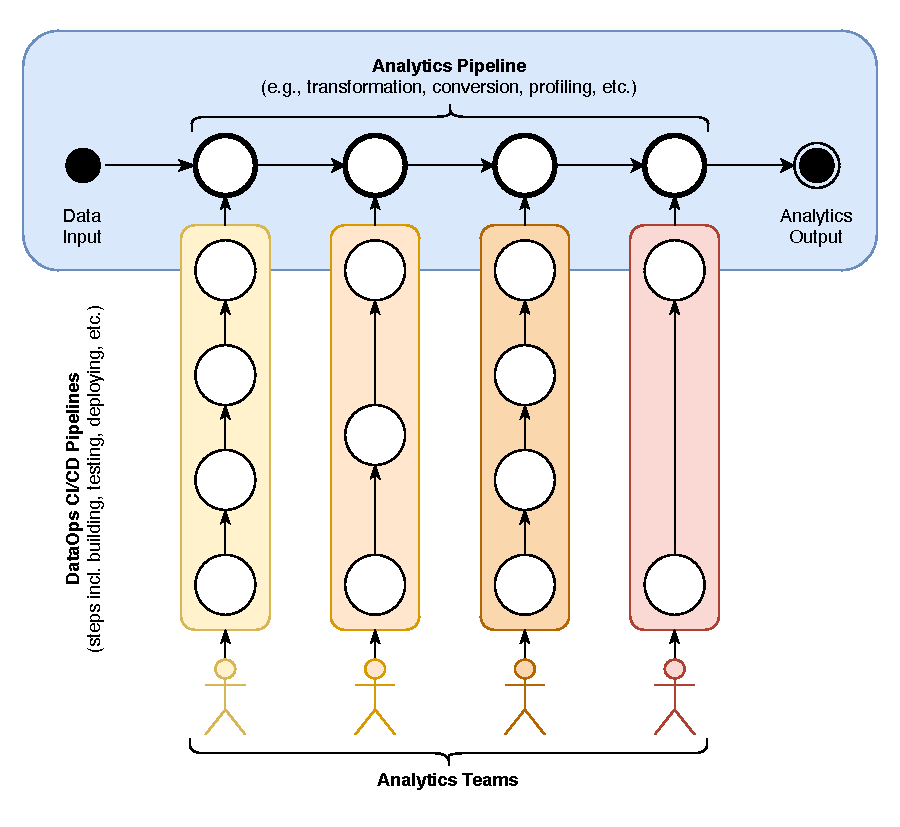
\includegraphics[width=\linewidth]{main-matter/img/2-1-2-pipeline-duality.pdf}
	\caption[DataOps Pipeline Duality]{DataOps Pipeline Duality (per \cite[38\psqq]{Bergh2019})}
	\label{fig:2-pipeline-duality}
\end{figure}

The data analytics (or data operations) pipeline is also called \textit{Value Pipeline} since it is in charge of answering questions through analytical insights \cite[32\psq]{Bergh2019}. Its horizontal representation visualizes its continuous flow. On the contrary, the vertical pipelines, also called \textit{Innovation Pipelines} represent the DataOps \ac{cicd} pipelines \cite[66]{Schmidt2019}. Whenever a new feature is developed for any stage of the pipeline, a number of preliminary steps is performed before finally deploying the solution into production \cite[33]{Bergh2019}. As with data analytics in general, the design of such pipelines highly depends on the analytics and quality requirements. In the scenario of Figure \ref{fig:2-pipeline-duality}, the individual stages require different \ac{cicd} steps and might also be worked on by different teams within the superordinate project.

As with DevOps, DataOps \ac{cicd} ties in with the project's \acf{vcs}. This allows for collaboration between developers as well as development environment management \cite{Davis2020}. Usually, a developer uses an individual sandbox to make changes to the common source code. This sandbox is a highly isolated environment which can be used without impacting the development process of other developers. It includes the current common source code as well as processes for installing and running all required dependencies \cite[41]{Bergh2019}. When committing a change to the \ac{vcs}, it triggers the corresponding \ac{cicd} pipeline which performs its checks and reports potential issues. Otherwise, the updated source code becomes the new common source code since the deployment into production has been conducted successfully.

Another methodology originating from DevOps is \textit{\ac{iac}}. In a desired automated environment, \ac{iac} also enables automatic creation, provisioning, and re-instantiation of a (cloud) infrastructure \cite[8\psqq]{Chaganti2018} which does not require repeated \ac{ui}-based configuration, etc. This is enabled by programatic configuration of infrastructure resources, settings, as well as applications.

\subsection{Agile Heritage: Fast-Paced, Iterative Development}
One problem within data analytics is that traditionally developed solutions cannot keep up with the demand of changing requirements. The development process is slow such that valuable and time-dependent information cannot be processed on time \cite{Lockner2019}. In software development, agile development mostly replaced traditional waterfall-orientated processes. \textit{Agile} in DataOps context means that development and improvement is iterative and fast-paced. It requires a \ac{mvp} which is continuously improved by means of previously mentioned \ac{spc} and \ac{cicd} processes \cite[19\psq]{Bergh2019}.
